\usetikzlibrary{arrows.meta,calc,patterns}

\begin{frame}{split caches; multiple cores}
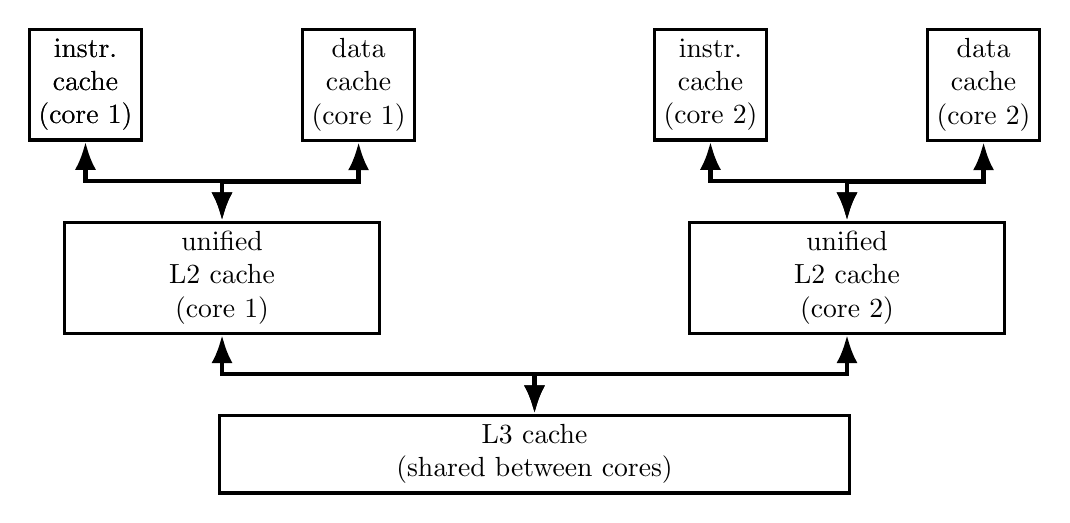
\begin{tikzpicture}
    \tikzset{
        >=Latex,
        connect/.style={<->,ultra thick},
        cache/.style={draw,very thick,align=center},
    }
\node[cache] (icache1) {instr. \\ cache \\ (core 1)};
\node[cache,anchor=west] (dcache1) at ([xshift=2cm]icache1.east) {data \\ cache \\ (core 1)};
\node[cache] (icache2) {instr. \\ cache \\ (core 1)};
\node[cache,anchor=west] (icache2) at ([xshift=3cm]dcache1.east) {instr. \\ cache \\ (core 2)};
\node[cache,anchor=west] (dcache2) at ([xshift=2cm]icache2.east) {data \\ cache \\ (core 2)};
\node[cache, minimum width=4cm,anchor=north] (l21) at ([yshift=-1cm]$(icache1.south)!0.5!(dcache1.south)$) {unified \\ L2 cache \\ (core 1)};
\node[cache, minimum width=4cm,anchor=north] (l22) at ([yshift=-1cm]$(icache2.south)!0.5!(dcache2.south)$) {unified \\ L2 cache \\ (core 2)};
    \node[cache, minimum width=8cm,anchor=north] (l3) at ([yshift=-1cm]$(l21.south)!0.5!(l22.south)$) {L3 cache \\ (shared between cores)};
\foreach \fromC/\toC in {icache1/l21,dcache1/l21,icache2/l22,dcache2/l22,l21/l3,l22/l3} {
\draw[connect] (\fromC.south) -- ++(-0cm,-.5cm) -| (\toC.north);
}
\end{tikzpicture}
\end{frame}

\begin{frame}{hierarchy and instruction/data caches}
    \begin{itemize}
    \item typically separate data and instruction caches for L1
    \vspace{.5cm}
    \item (almost) never going to read instructions as data or vice-versa
    \item avoids instructions evicting data and vice-versa
    \item can optimize instruction cache for different access pattern
    \item easier to build fast caches: that handles less accesses at a time
    \end{itemize}
\end{frame}

